\documentclass[12pt, letterpaper, titlepage, hidelinks]{article}

% Packages
\usepackage[letterpaper, margin=1in]{geometry}
\usepackage[utf8]{inputenc}
\usepackage{fancyhdr}
\usepackage{setspace}
\usepackage{amssymb}
\usepackage{amsmath}
\usepackage{multirow}
\usepackage{array}
\usepackage{graphicx}
\usepackage{tabularx}
\usepackage{booktabs}
\usepackage{hyperref}
\usepackage{scrextend}
\usepackage{verbatim}
\usepackage[english]{babel}
\usepackage{blindtext}
\usepackage{capt-of}
\usepackage{float}
\usepackage{caption}
\usepackage{apacite}
\usepackage{mathrsfs}
\usepackage{pdfpages}
\usepackage[autostyle, english = american]{csquotes}
\MakeOuterQuote{"}

\graphicspath{ {Images/} }


\newenvironment{nospaceflalign*}
{\setlength{\abovedisplayskip}{0px}\setlength{\belowdisplayskip}{0px}%
	\csname flalign*\endcsname}
{\csname endflalign*\endcsname\ignorespacesafterend}

% Title Page
\title{4DM4 Lab 1 Report \\ Linear Feedback Shift Register}
\author{Ashpan Raskar raskara 400185326\\
		Ahnaf Bhuiyan bhuiya3 400198359}
\date{\today}



\begin{document}

\maketitle
\tableofcontents
\newpage
\setlength{\parindent}{0pt}
\setcounter{secnumdepth}{0}
\section{Part A}
	\subsection{A2}
		Yes, the Linear Feedback Shift Register (LFSR) does reach a steady state. It takes 4194303 ($\approx$4.19 million) clock ticks for the LFSR to return back to its original state. This is also known as the period of the output stream.
	\subsection{A3}
		Included at the end of the file is the first page of the randomly generated numbers from the LFSR\@.
	\subsection{A4}
		The formula for the conditional probability of a 0-run and a 1-run of length k occuring is given by:
		\begin{equation}
			{(\frac{1}{2})}^{k}
		\end{equation}
		Ideally the LFSR is used to create a perfectly random number using binary strings which are then converted to decimal. For a binary string to be completely random, each digit in the string must have a 50\% chance of being a 1, and 50\% chance for being a 0. The formula we have given follows this justification. For example, since a digit has a 50\% chance to be a 1. Any consecutive digits after will also have a 50\% chance of being 1, individually. Therefore for 1-run to be 3 digits long the probability can be calculated as such:
		\begin{equation}
			\frac{1}{2} * \frac{1}{2} * \frac{1}{2}
		\end{equation}
		The same probablility can be applied to a 0-run. This means for any 1-run or 0-run of k-length, the theoretical probability can be calculated by the formula given in (1).
	\subsection{A5}
		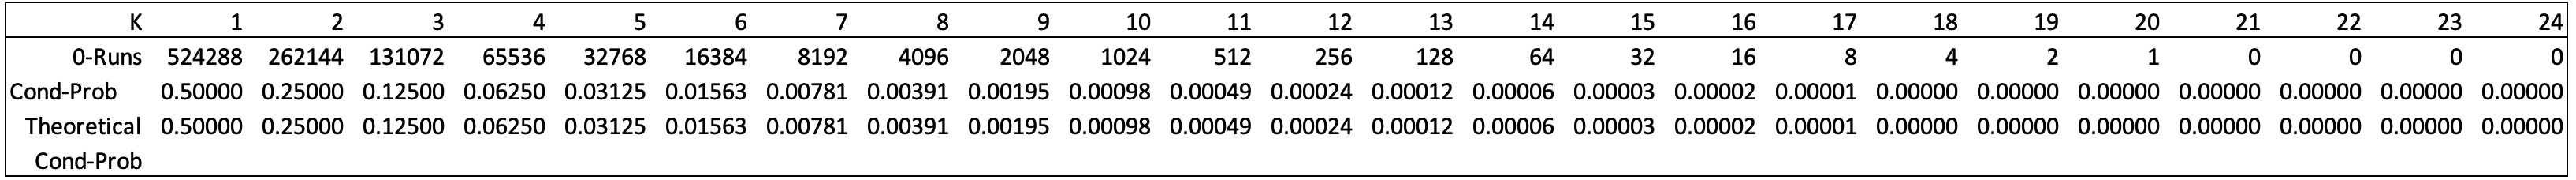
\includegraphics[width=\textwidth]{0_run_table}
		Table 1: Table of 0-run lengths and their probabilities.
	\subsection{A6}
		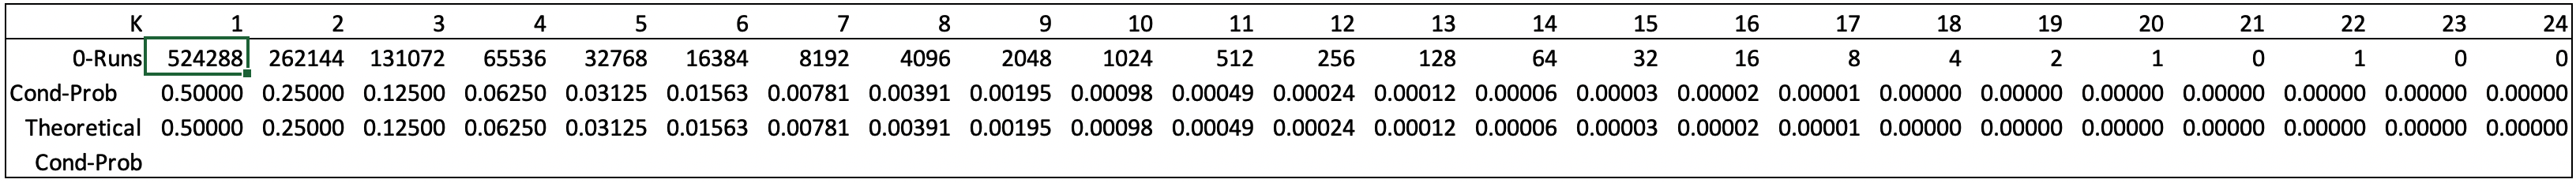
\includegraphics[width=\textwidth]{1_run_table}
		Table 2: Table of 1-run lengths and their probabilities.
\section{Part B}
		\subsection{B2}
			\begin{enumerate}
				\item The space delimted file of random numbers was saved to a vector variable in matlab. This vector was of size 1$\times$524287.
				\item Then a triple nested for loop was used to iterate through the dimensions rows, columns, and depth from the image to be encrypted. In our case the dimensions were $427\times640\times8$. For the \verb|RAND_matrix| vector of those dimensions, for every cycle in the loop, a random number was selected from the vector that has all the random numbers. In our case we did run out of random numbers, so we had to loop back from the random numbers vector. It is noted that doing so invalidates Shannon's One Time PAD principle, but this was done for ease of implementation, as increasing the size of the LFSR is very computationally heavy.
			\end{enumerate}
		\subsection{B3}
			The \verb|RAND_matrix| was then used to XOR the image with the image vector \verb|A| to encrypt the image. The encrypted image was then saved to a file.
			\begin{enumerate}
				\item First every element in the \verb|RAND_matrix| vector was visited.
				\item Then the function \verb|bitxor| was used to XOR the \verb|RAND_matrix| element with the corresponding element in the image vector \verb|A|.
				\item The result was then saved to the \verb|A_encrypted| vector.
				\item Finally the \verb|A_encrypted| vector was displayed as an image using \verb|image(uint8(A_encrypted))|.
			\end{enumerate}
		\subsection{B4}
			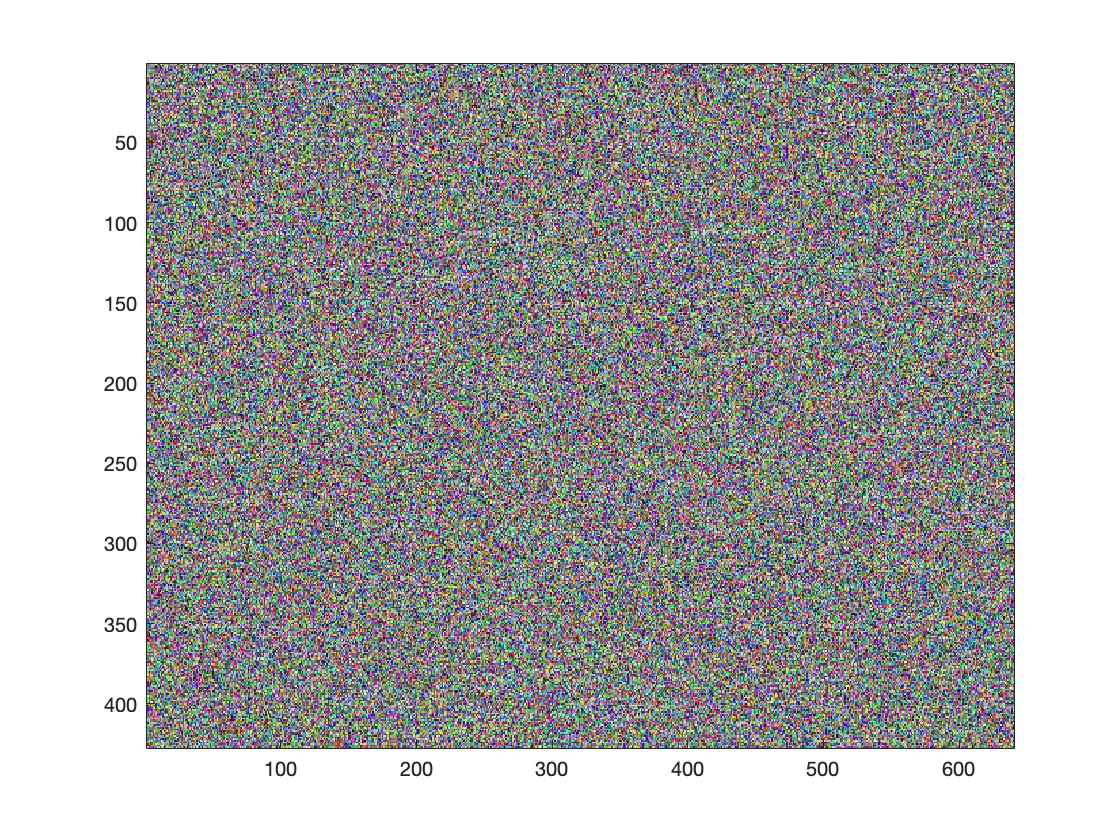
\includegraphics[width=0.45\textwidth]{encrypted_image} \newline
			Figure 1: Encrypted image generated by XORing the \verb|RAND_matrix| and image vectors.
		\subsection{B5}
			\begin{enumerate}
				\item First every element in the \verb|RAND_matrix| vector was visited.
				\item Then the function \verb|bitxor| was used to XOR the \verb|RAND_matrix| element with the corresponding element in the encrypted image vector \verb|A_encrypted|.
				\item The result was then saved to the \verb|A_decrypted| vector.
				\item Finally the \verb|A_decrypted| vector was displayed as an image using \verb|image(uint8(A_decrypted))|.
			\end{enumerate}
			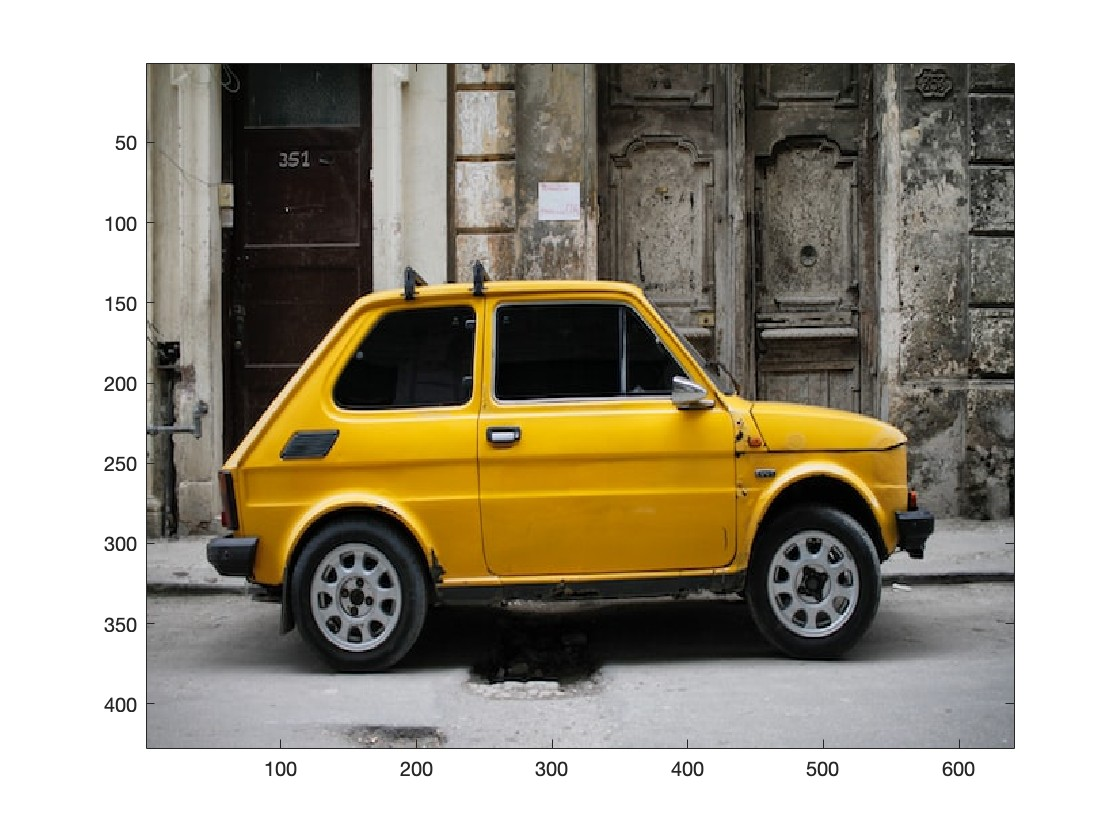
\includegraphics[width=0.45\textwidth]{decrypted_image} \newline
			Figure 2: Decrypted image generated by XORing the \verb|RAND_matrix| and \verb|A_encrypted| vectors.
\section{Extra Info}
	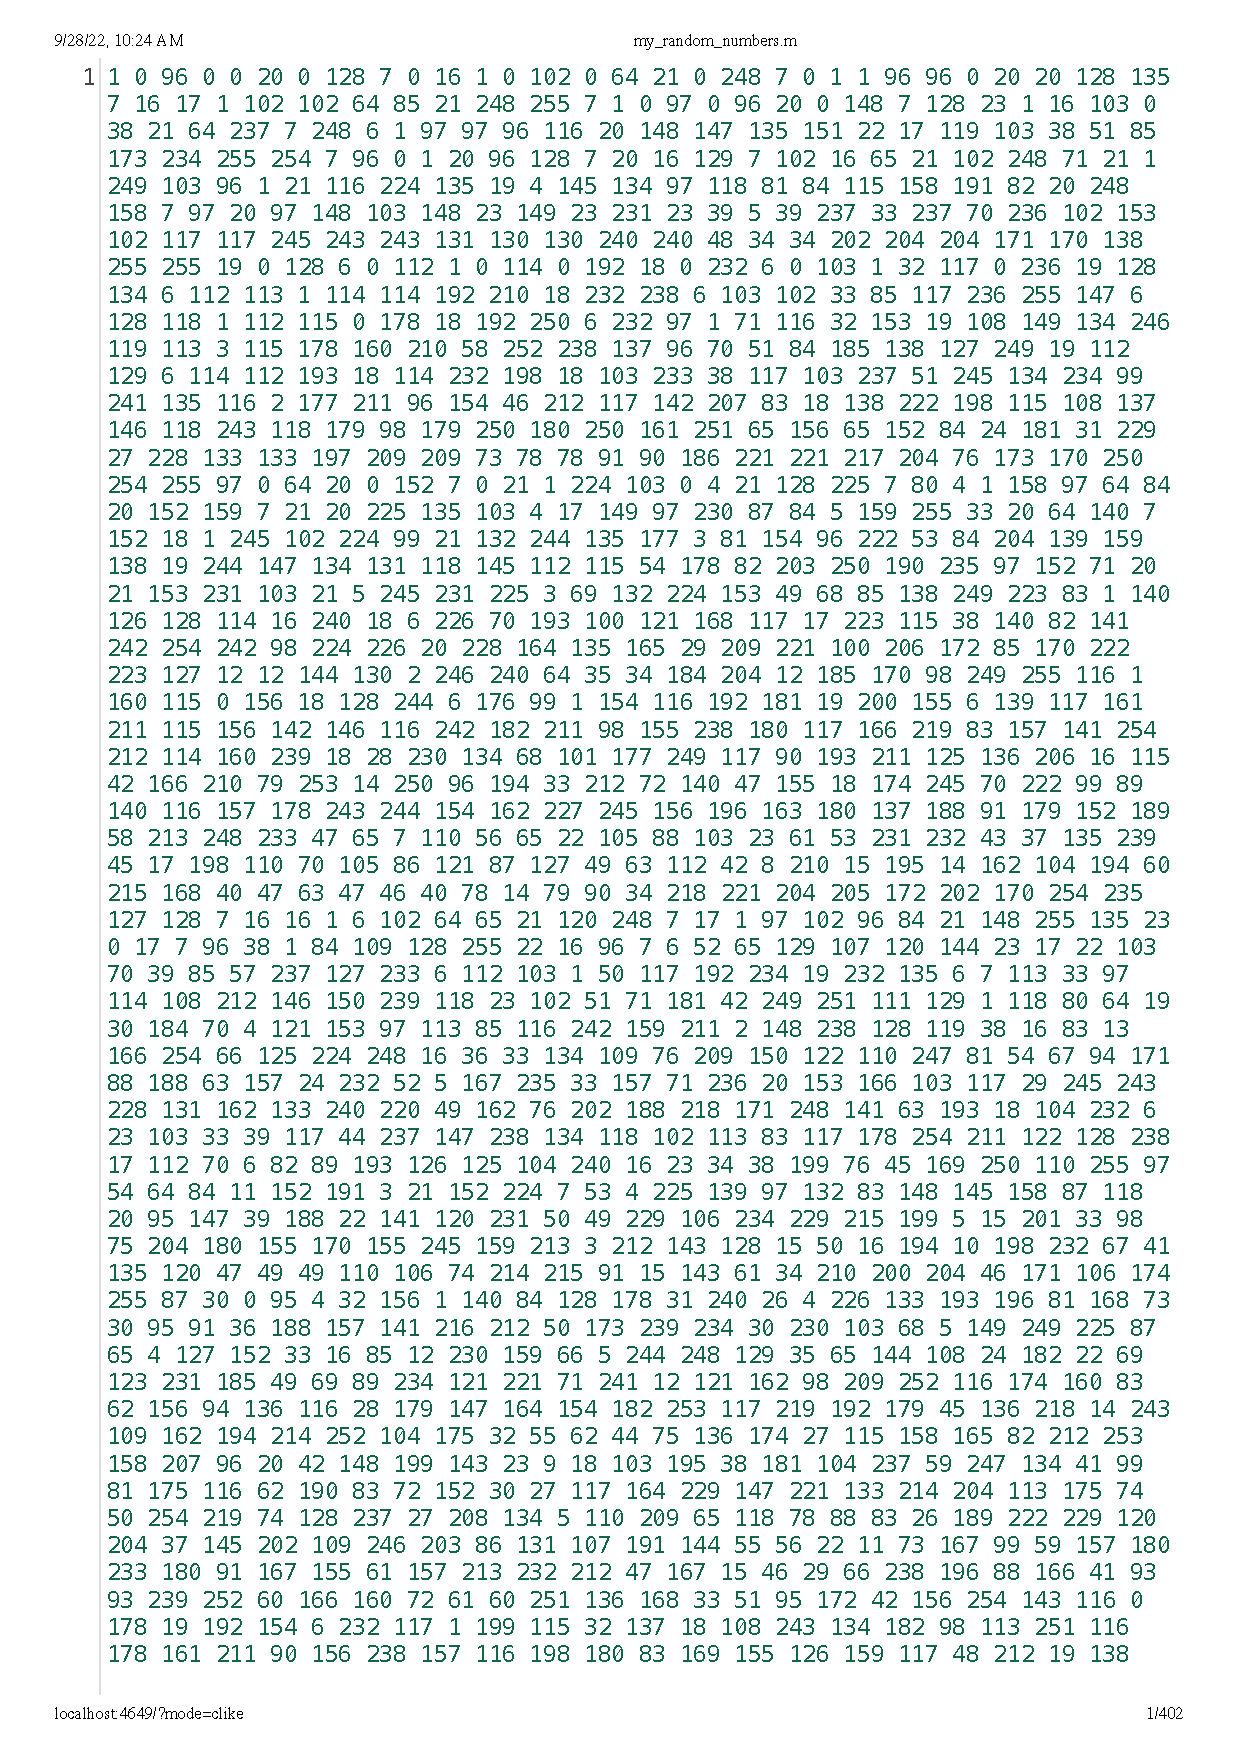
\includepdf[pages=-]{my_random_numbers.pdf}
	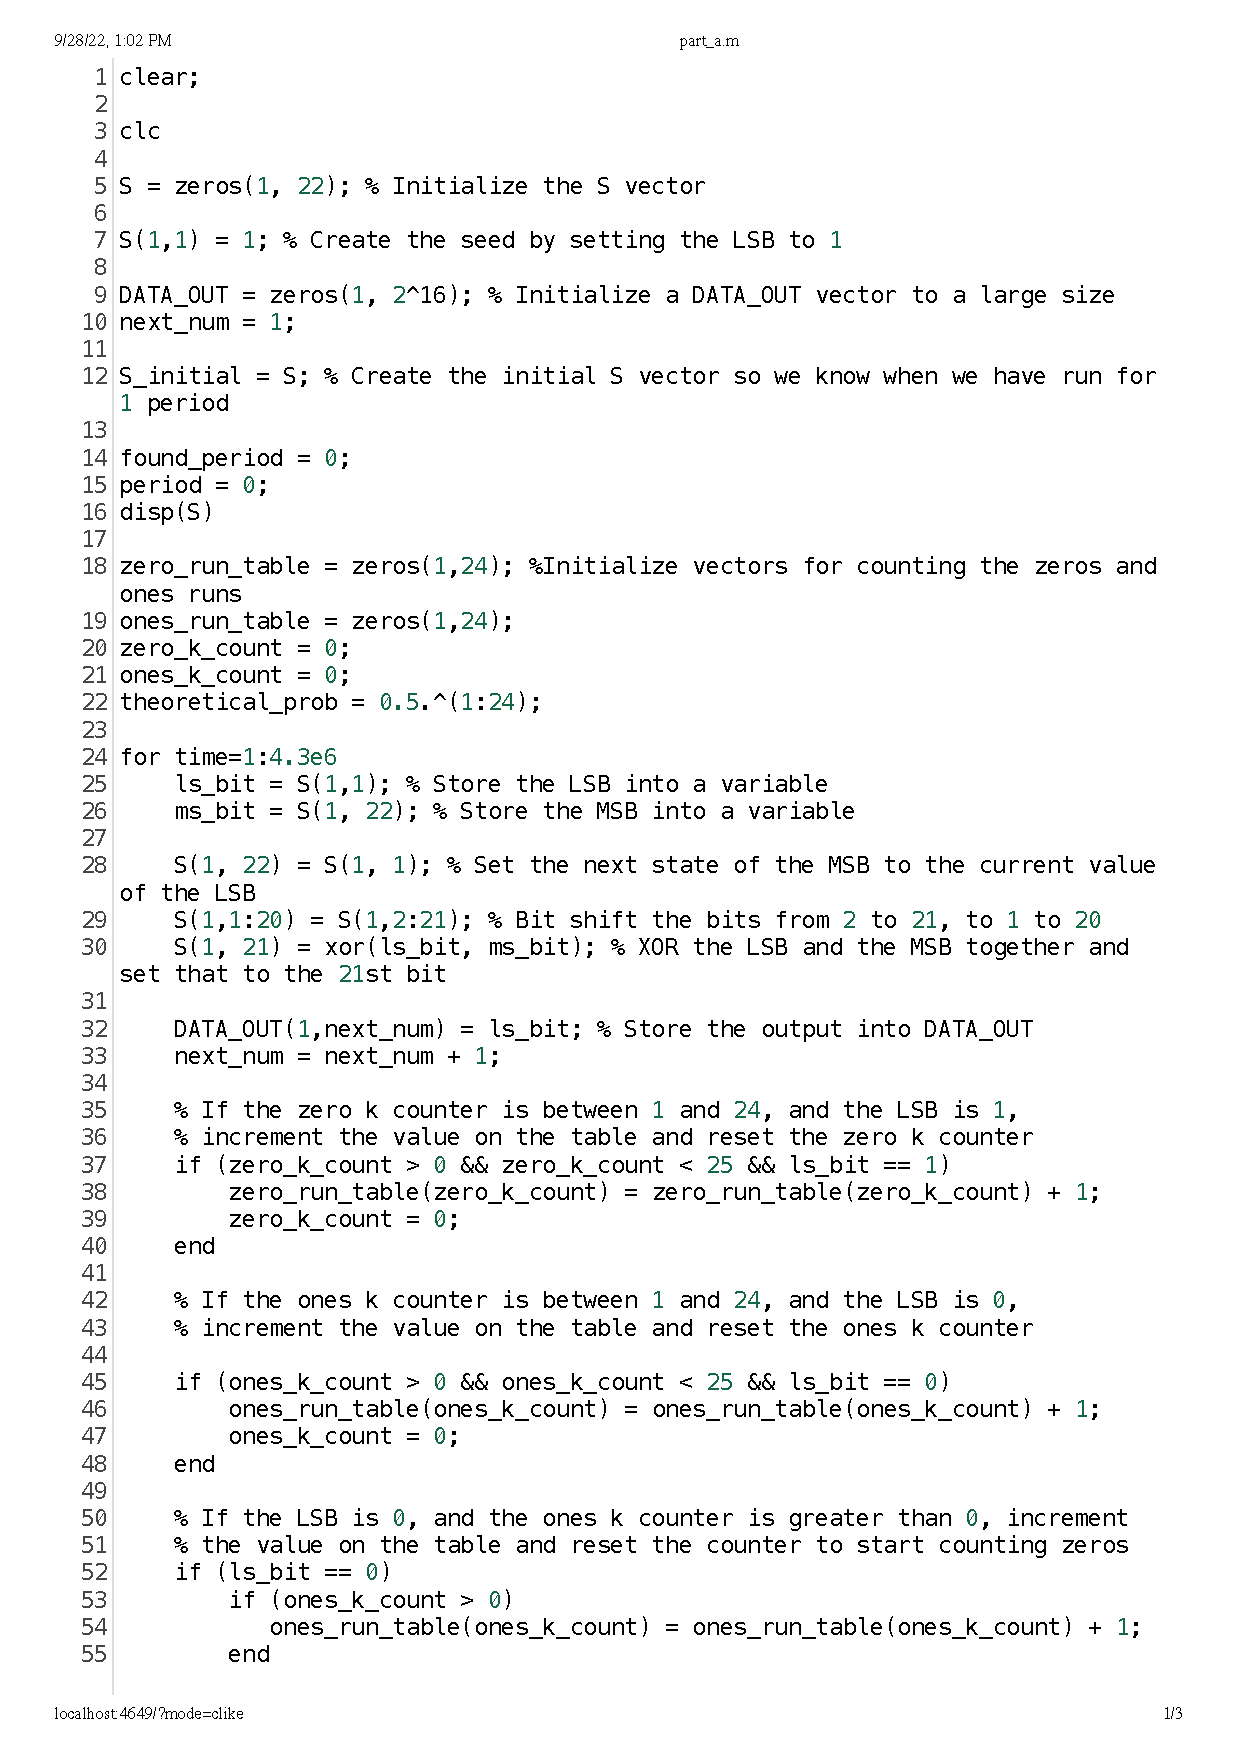
\includepdf[pages=-]{part_a.pdf}
	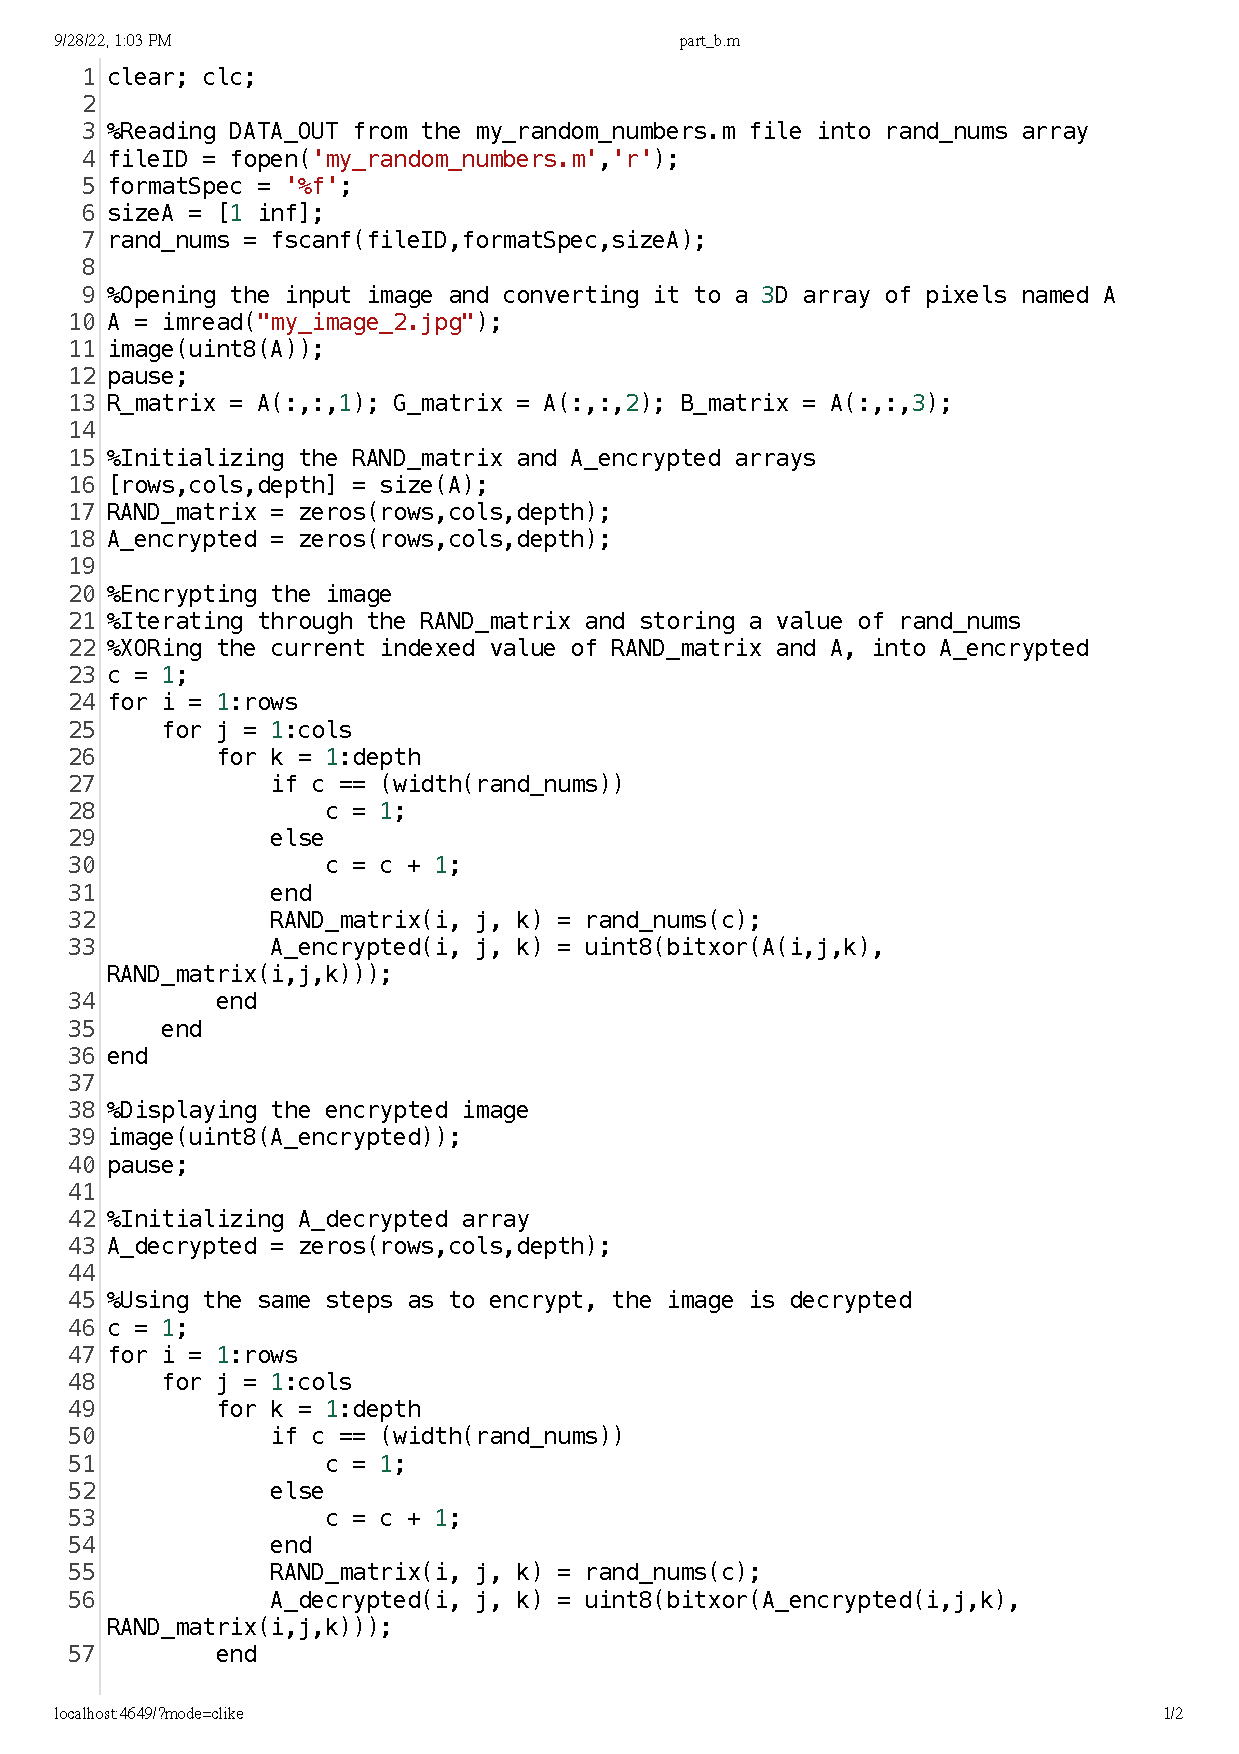
\includepdf[pages=-]{part_b.pdf}
\end{document}          